% Graphic for TeX using PGF
% Title: C:\Users\Hugo\Dropbox\PUC\Disciplinas\PM\Material\Tex\programacao-modular-2016-1-04-classes-e-encapsulamento\classeUML.dia
% Creator: Dia v0.97.2
% CreationDate: Sat Aug 13 00:13:02 2016
% For: Hugo
% \usepackage{tikz}
% The following commands are not supported in PSTricks at present
% We define them conditionally, so when they are implemented,
% this pgf file will use them.
\ifx\du\undefined
  \newlength{\du}
\fi
\setlength{\du}{15\unitlength}
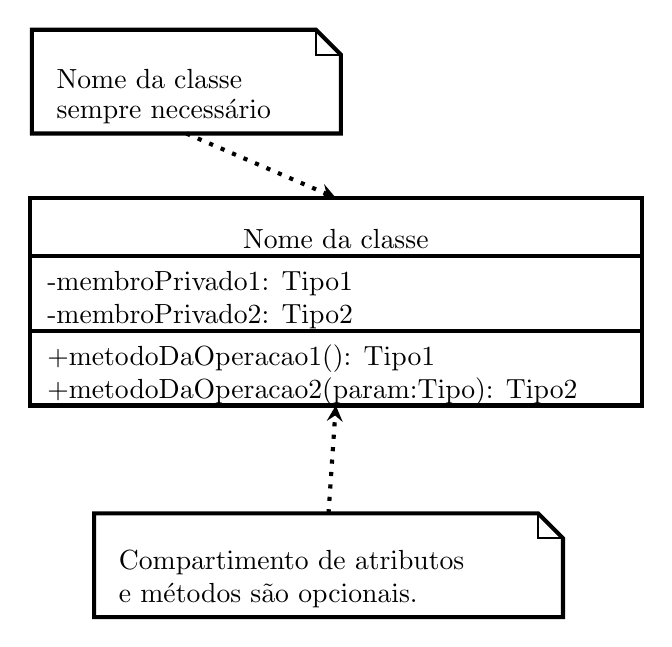
\begin{tikzpicture}
\pgftransformxscale{1.000000}
\pgftransformyscale{-1.000000}
\definecolor{dialinecolor}{rgb}{0.000000, 0.000000, 0.000000}
\pgfsetstrokecolor{dialinecolor}
\definecolor{dialinecolor}{rgb}{1.000000, 1.000000, 1.000000}
\pgfsetfillcolor{dialinecolor}
\pgfsetlinewidth{0.100000\du}
\pgfsetdash{}{0pt}
\definecolor{dialinecolor}{rgb}{1.000000, 1.000000, 1.000000}
\pgfsetfillcolor{dialinecolor}
\fill (15.750000\du,4.900000\du)--(15.750000\du,6.300000\du)--(30.495000\du,6.300000\du)--(30.495000\du,4.900000\du)--cycle;
\definecolor{dialinecolor}{rgb}{0.000000, 0.000000, 0.000000}
\pgfsetstrokecolor{dialinecolor}
\draw (15.750000\du,4.900000\du)--(15.750000\du,6.300000\du)--(30.495000\du,6.300000\du)--(30.495000\du,4.900000\du)--cycle;
% setfont left to latex
\definecolor{dialinecolor}{rgb}{0.000000, 0.000000, 0.000000}
\pgfsetstrokecolor{dialinecolor}
\node at (23.122500\du,5.900000\du){Nome da classe};
\definecolor{dialinecolor}{rgb}{1.000000, 1.000000, 1.000000}
\pgfsetfillcolor{dialinecolor}
\fill (15.750000\du,6.300000\du)--(15.750000\du,8.100000\du)--(30.495000\du,8.100000\du)--(30.495000\du,6.300000\du)--cycle;
\definecolor{dialinecolor}{rgb}{0.000000, 0.000000, 0.000000}
\pgfsetstrokecolor{dialinecolor}
\draw (15.750000\du,6.300000\du)--(15.750000\du,8.100000\du)--(30.495000\du,8.100000\du)--(30.495000\du,6.300000\du)--cycle;
% setfont left to latex
\definecolor{dialinecolor}{rgb}{0.000000, 0.000000, 0.000000}
\pgfsetstrokecolor{dialinecolor}
\node[anchor=west] at (15.900000\du,6.960000\du){-membroPrivado1: Tipo1};
% setfont left to latex
\definecolor{dialinecolor}{rgb}{0.000000, 0.000000, 0.000000}
\pgfsetstrokecolor{dialinecolor}
\node[anchor=west] at (15.900000\du,7.760000\du){-membroPrivado2: Tipo2};
\definecolor{dialinecolor}{rgb}{1.000000, 1.000000, 1.000000}
\pgfsetfillcolor{dialinecolor}
\fill (15.750000\du,8.100000\du)--(15.750000\du,9.900000\du)--(30.495000\du,9.900000\du)--(30.495000\du,8.100000\du)--cycle;
\definecolor{dialinecolor}{rgb}{0.000000, 0.000000, 0.000000}
\pgfsetstrokecolor{dialinecolor}
\draw (15.750000\du,8.100000\du)--(15.750000\du,9.900000\du)--(30.495000\du,9.900000\du)--(30.495000\du,8.100000\du)--cycle;
% setfont left to latex
\definecolor{dialinecolor}{rgb}{0.000000, 0.000000, 0.000000}
\pgfsetstrokecolor{dialinecolor}
\node[anchor=west] at (15.900000\du,8.760000\du){+metodoDaOperacao1(): Tipo1};
% setfont left to latex
\definecolor{dialinecolor}{rgb}{0.000000, 0.000000, 0.000000}
\pgfsetstrokecolor{dialinecolor}
\node[anchor=west] at (15.900000\du,9.560000\du){+metodoDaOperacao2(param:Tipo): Tipo2};
\pgfsetlinewidth{0.100000\du}
\pgfsetdash{}{0pt}
\definecolor{dialinecolor}{rgb}{1.000000, 1.000000, 1.000000}
\pgfsetfillcolor{dialinecolor}
\fill (15.800000\du,0.850000\du)--(22.645000\du,0.850000\du)--(23.245000\du,1.450000\du)--(23.245000\du,3.350000\du)--(15.800000\du,3.350000\du)--cycle;
\definecolor{dialinecolor}{rgb}{0.000000, 0.000000, 0.000000}
\pgfsetstrokecolor{dialinecolor}
\draw (15.800000\du,0.850000\du)--(22.645000\du,0.850000\du)--(23.245000\du,1.450000\du)--(23.245000\du,3.350000\du)--(15.800000\du,3.350000\du)--cycle;
\pgfsetlinewidth{0.050000\du}
\definecolor{dialinecolor}{rgb}{0.000000, 0.000000, 0.000000}
\pgfsetstrokecolor{dialinecolor}
\draw (22.645000\du,0.850000\du)--(22.645000\du,1.450000\du)--(23.245000\du,1.450000\du);
% setfont left to latex
\definecolor{dialinecolor}{rgb}{0.000000, 0.000000, 0.000000}
\pgfsetstrokecolor{dialinecolor}
\node[anchor=west] at (16.150000\du,2.032500\du){Nome da classe };
% setfont left to latex
\definecolor{dialinecolor}{rgb}{0.000000, 0.000000, 0.000000}
\pgfsetstrokecolor{dialinecolor}
\node[anchor=west] at (16.150000\du,2.832500\du){sempre necessário};
\pgfsetlinewidth{0.100000\du}
\pgfsetdash{}{0pt}
\definecolor{dialinecolor}{rgb}{1.000000, 1.000000, 1.000000}
\pgfsetfillcolor{dialinecolor}
\fill (17.300000\du,12.500000\du)--(27.995000\du,12.500000\du)--(28.595000\du,13.100000\du)--(28.595000\du,15.000000\du)--(17.300000\du,15.000000\du)--cycle;
\definecolor{dialinecolor}{rgb}{0.000000, 0.000000, 0.000000}
\pgfsetstrokecolor{dialinecolor}
\draw (17.300000\du,12.500000\du)--(27.995000\du,12.500000\du)--(28.595000\du,13.100000\du)--(28.595000\du,15.000000\du)--(17.300000\du,15.000000\du)--cycle;
\pgfsetlinewidth{0.050000\du}
\definecolor{dialinecolor}{rgb}{0.000000, 0.000000, 0.000000}
\pgfsetstrokecolor{dialinecolor}
\draw (27.995000\du,12.500000\du)--(27.995000\du,13.100000\du)--(28.595000\du,13.100000\du);
% setfont left to latex
\definecolor{dialinecolor}{rgb}{0.000000, 0.000000, 0.000000}
\pgfsetstrokecolor{dialinecolor}
\node[anchor=west] at (17.650000\du,13.682500\du){Compartimento de atributos };
% setfont left to latex
\definecolor{dialinecolor}{rgb}{0.000000, 0.000000, 0.000000}
\pgfsetstrokecolor{dialinecolor}
\node[anchor=west] at (17.650000\du,14.482500\du){e métodos são opcionais.};
\pgfsetlinewidth{0.100000\du}
\pgfsetdash{{\pgflinewidth}{0.200000\du}}{0cm}
\pgfsetdash{{\pgflinewidth}{0.200000\du}}{0cm}
\pgfsetbuttcap
{
\definecolor{dialinecolor}{rgb}{0.000000, 0.000000, 0.000000}
\pgfsetfillcolor{dialinecolor}
% was here!!!
\pgfsetarrowsend{stealth}
\definecolor{dialinecolor}{rgb}{0.000000, 0.000000, 0.000000}
\pgfsetstrokecolor{dialinecolor}
\draw (19.522500\du,3.350000\du)--(23.122500\du,4.900000\du);
}
\pgfsetlinewidth{0.100000\du}
\pgfsetdash{{\pgflinewidth}{0.200000\du}}{0cm}
\pgfsetdash{{\pgflinewidth}{0.200000\du}}{0cm}
\pgfsetbuttcap
{
\definecolor{dialinecolor}{rgb}{0.000000, 0.000000, 0.000000}
\pgfsetfillcolor{dialinecolor}
% was here!!!
\pgfsetarrowsend{stealth}
\definecolor{dialinecolor}{rgb}{0.000000, 0.000000, 0.000000}
\pgfsetstrokecolor{dialinecolor}
\draw (22.947500\du,12.500000\du)--(23.122500\du,9.900000\du);
}
\end{tikzpicture}
